\documentclass[a4paper, 12pt]{article}

\usepackage{polski}
\usepackage[utf8]{inputenc}
\usepackage{a4wide}
\usepackage[OT4]{fontenc}
\usepackage[english,polish]{babel}
\usepackage{indentfirst}
\usepackage{graphicx} 
\usepackage{float}
\usepackage{listings}
\usepackage[hidelinks, pdftoolbar = false, pdfmenubar = false, bookmarks = false]{hyperref}
\usepackage{geometry}
    
\renewcommand{\baselinestretch}{1.0}
\newgeometry{tmargin=2.5cm, bmargin=2.5cm, lmargin=2.5cm, rmargin=2.5cm} 
    
\begin{document}

\thispagestyle{empty}
\noindent Aleksander Prus, 218404 \hfill Wrocław, d.\ \today
\\ Rafał Szyszka, 218207

\vfill

\begin{center}
    \begin{Huge}
        Monte Carlo Tree Search\\
    \end{Huge}
\end{center}

\begin{center}
    Rok akad. 2017/2018, DAN
\end{center}

\vspace{0.2ex}

\begin{flushright}
    \begin{minipage}[t]{0.4\columnwidth}
        \noindent Mgr inż. Jan Jakubik
    \end{minipage}
\end{flushright}

\vfill
\newpage
\tableofcontents
%%%%%%%%%%%%%%%%%%%%%%%%%%%%%%%%%%%%%%%%%%%%%%%%%%%%%%%%%%%%%%%%%%%%%%%%%%%%%%%%%%%%%%%%%%%%%%%%%%%%%%%%%%%%%%%%%%%%%%%%%%%%%%%%%%%%%%%%%%%%%%%%%%%%%%%%%%%%
\newpage
\section{Cel ćwiczenia}
Celem ćwiczenia była iplementacja uproszczonej wersji popularnej gry Hearthstone, z graczem komputerowym, którego zachowanie zdefiniowane będzie algorytmem Monte Carlo Tree Search. Dodatkowo należało zaimplementować trzech graczy naiwnych:
\begin{itemize}
\item losowy,
\item agresywny,
\item kontrolujący.
\end{itemize}

Gracz agresywny w pierwszej kolejności skupia się na zadaniu jak największej ilości obrażeń bohaterowi gracza. Natomiast gracz kontrolujący skupia się na wyeliminowaniu minionów przeciwnika.


\section{Realizacja}
Do realizacji zadania wybrano język Python, ze względu na mnogość zewnętrznych bibliotek oraz wysoki poziom abstrakcji języka.

\subsection{Naiwni gracze}
Logika naiwnych graczy została zimplementowana w pakiecie \textbf{naive-bots}. Ich zachowanie określają dwie metody \textbf{card-rating} oraz \textbf{choose-targets}. Pierwsza z nich odpowiada za dobór kart do zagrania z ręki, w turze wybrangeo bota. Natomiast druga metoda, odpowiada za wybór celów do zaatakowania po stronie przeciwnika.

\subsubsection{Gracz losowy}
Ten gracz w sposób losowy wybiera karty do zagrania oraz cele, które zaatakuje w danej turze.

\subsubsection{Gracz agresywny}
Ten gracz preferuje karty z dużą ilością ataku. Za swoje cele, w pierwszej kolejności, bierze karty przeciwnika z właściwością \textbf{[TAUNT]}, następnie wybiera karty z wysoką wartością życia (większy od 4), jeżeli takich kart przeciwnik nie posiada na stole, bot agresywny atakuje jego bohatera.

\subsubsection{Gracz kontrolujący}
Ten gracz preferuje karty defensywne, z dużą ilością życia. Za swoje cele, w pierwszej kolejności, bierze karty przeciwnika z właściwością \textbf{[TAUNT]}, następnie wybiera karty z wysoką wartością życia (większy od 4), następnie wybiera pozostałe karty przeciwnika na stole. Bohater przeciwnika jest ostatnim wybieranym celem gracza kontrolującego.

\subsection{Gracz Monte Carlo}
Jego działanie opiera się na czterech krokach budowy drzewa decyzyjnego:
\begin{itemize}
\item wybór,
\item rozrost,
\item symulacja,
\item propagacja wstecz.
\end{itemize}
Te cztery kroki są wykonywane dopóki czas przydzielony na wykonanie ruchu nie upłynie. Następnie wybierany jest ruch z korzenia drzewa, dla ktorego została wykonana największa liczba symulacji.

\section{Badania}
Łącznie rozegrano sześć potyczek, trzy dla gracza Monte Carlo z maksymalnym czasem na ruch wynoszącym 20 sekund i trzy dla gracza Monte Carlo z maksymalnym czasem na ruch wynoszącym 60 sekund.

Gracz Monte Carlo grał z każdym z naiwnych graczy stukrotnie dla obu ustawianień czasowych. Wyniki zaprezentowano poniżej. 

\begin{figure}[H]
	\centering
	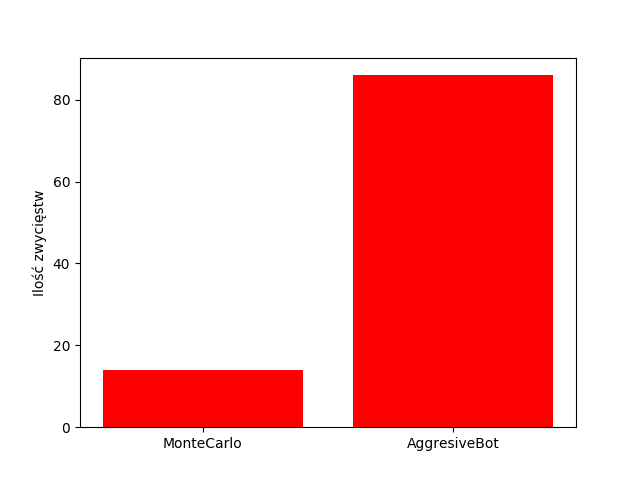
\includegraphics[scale=0.75]{20-100_a_vs_m.png}
	\caption{Monte Carlo versus Gracz Agresywny, 100 rozgrywek, 20 sekund na ruch}
\end{figure}

\begin{figure}[H]
	\centering
	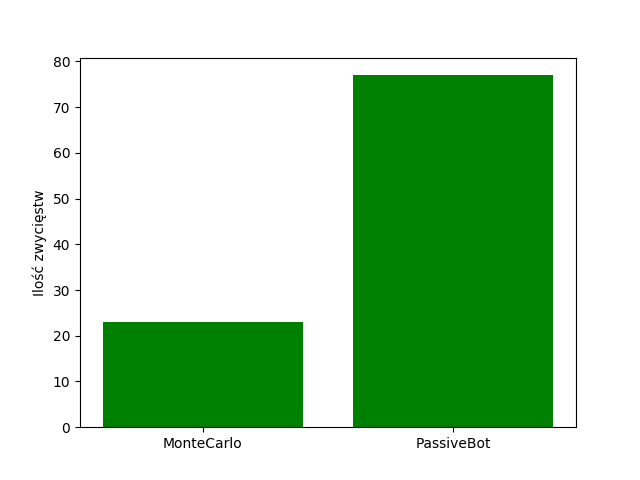
\includegraphics[scale=0.75]{20-100_p_vs_m.png}
	\caption{Monte Carlo versus Gracz Kontrolujący, 100 rozgrywek, 20 sekund na ruch}
\end{figure}

\begin{figure}[H]
	\centering
	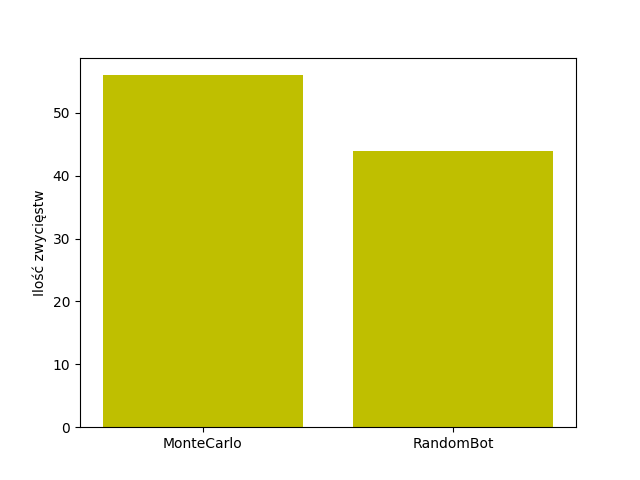
\includegraphics[scale=0.75]{20-100_r_vs_m.png}
	\caption{Monte Carlo versus Gracz Losowy, 100 rozgrywek, 20 sekund na ruch}
\end{figure}

\begin{figure}[H]
	\centering
	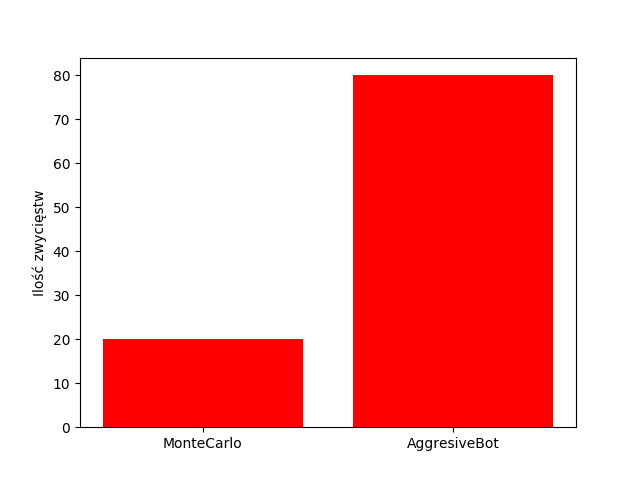
\includegraphics[scale=0.75]{60-100_a_vs_m.png}
	\caption{Monte Carlo versus Gracz Agresywny, 100 rozgrywek, 60 sekund na ruch}
\end{figure}

\begin{figure}[H]
	\centering
	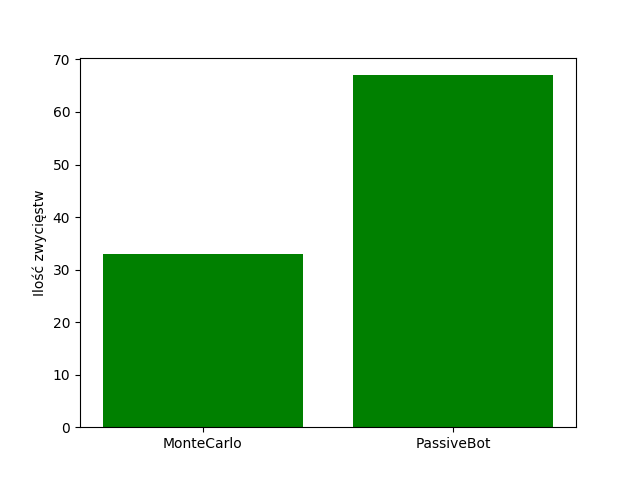
\includegraphics[scale=0.75]{60-100_p_vs_m.png}
	\caption{Monte Carlo versus Gracz Kontrolujący, 100 rozgrywek, 60 sekund na ruch}
\end{figure}

\begin{figure}[H]
	\centering
	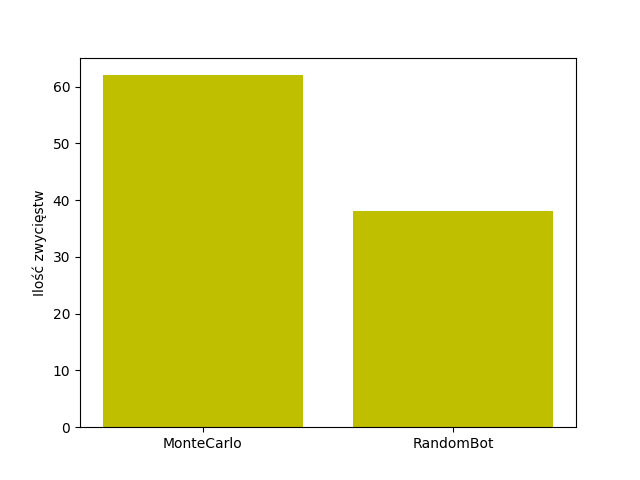
\includegraphics[scale=0.75]{60-100_r_vs_m.png}
	\caption{Monte Carlo versus Gracz Losowy, 100 rozgrywek, 60 sekund na ruch}
\end{figure}

Dodatkowo, dla porównania, rozegrano potyczki:
\begin{itemize}
\item Gracz Losowy versus Gracz Agresywny,
\item Gracz Losowy versus Gracz Pasywny,
\item Gracz Pasywny versus Gracz Agresywny.
\end{itemize}

Wyniki rozgrywek zaprezentowano na wykresach poniżej.

\begin{figure}[H]
	\centering
	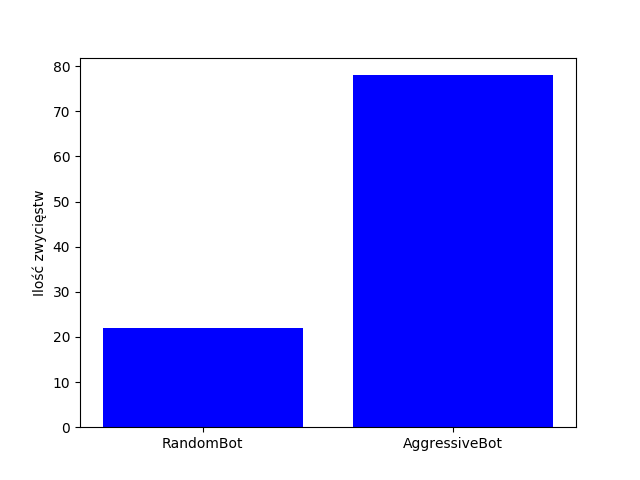
\includegraphics[scale=0.75]{100_r_vs_a.png}
	\caption{Gracz Losowy versus Gracz Agresywny, 100 rozgrywek}
\end{figure}

\begin{figure}[H]
	\centering
	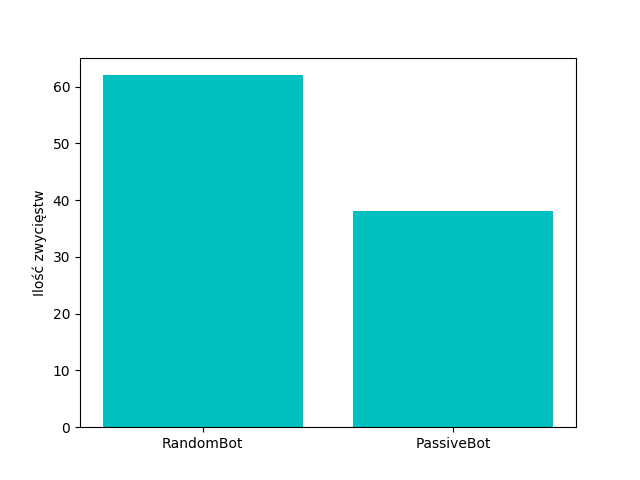
\includegraphics[scale=0.75]{100_r_vs_p.png}
	\caption{Gracz Losowy versus Gracz Kontrolujący, 100 rozgrywek}
\end{figure}

\begin{figure}[H]
	\centering
	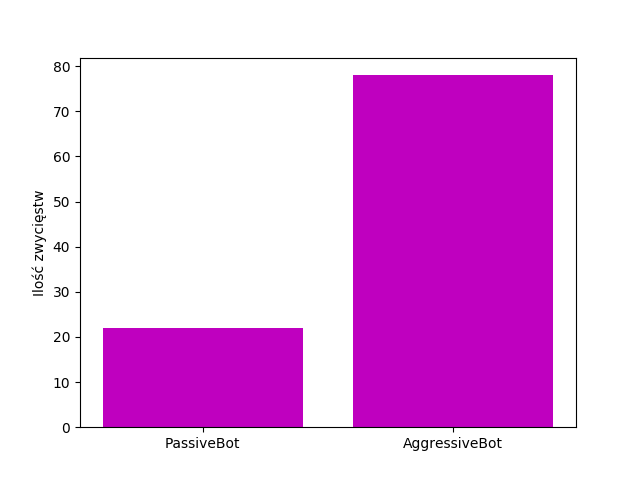
\includegraphics[scale=0.75]{100_p_vs_a.png}
	\caption{Gracz Kontrolujący versus Gracz Agresywny, 100 rozgrywek}
\end{figure}

\section{Wnioski}
Gracz Monte Carlo nie okazał się najlepszym graczem spośród tych zaimplementowanych. Jego 'jakość' uzależniona jest od czasu, jaki zostanie mu przydzielony na wykonanie ruchu. Dzieje się tak, ponieważ drzewo gry Hearthstone, nawet w wersji uproszczonej, jest bardzo duże i przejrzenie go w całości zajmuje wiele czasu. Znacznie prostszy w implementacji i szybciej działający gracz Agresywny okazał się być najlepiej grającym przeciwnikiem.

\end{document}